\documentclass[a4paper]{report}

\usepackage[utf8]{inputenc} %Accent
%\usepackage{libertine} %Font
\usepackage[english, francais]{babel} %langue

\usepackage{graphicx} %Include fig
\usepackage{caption} %center the caption
\usepackage{subfig} %Include subfig
\usepackage{lastpage} %ref LastPage 
\usepackage{fancyhdr} % headers,footers
\usepackage{multicol} % minipages
\usepackage{textcomp} 
\usepackage{lscape}   %Format paysage
\usepackage{fancybox} %Image arrière plan
\usepackage{amsmath} %\mathbb, \mathit...
\usepackage{amssymb} 
\usepackage{color} %couleurs
\usepackage{float}
\usepackage[hidelinks]{hyperref} %Liens intradoc et url
\usepackage{titlepic}
\usepackage{tikz} 
%\usepakcage{algorithm}
%\usepackage{algorithmic} %Algo en pseudo code
%\usepackage{algorithm2e} %for psuedo code

%\usepackage{boxedminipage} %Surligner

%\newcounter{apppage} % Annexes

%Dossier contenant les figures
\graphicspath{{../fig/}}

%Mise en page
\voffset -1.5 cm
\textheight 24.3 cm
\topmargin 0 cm
\headheight 0 cm
%\headsep 0.6 cm
\textwidth 16.5 cm
\evensidemargin 0 cm
\marginparsep 0 cm
\marginparwidth 0 cm
\oddsidemargin -.5 cm

%Titre
%\title{Speech Signal Processing\\Report\\Project n°2}
\newcommand{\horrule}[1]{\rule{\linewidth}{#1}} % Create horizontal rule command with 1 argument of height 
%\title{Final Report}

\title{	 
\textsc{EQ2320 - Speech Signal Processing}\\[25pt] 
\horrule{1pt} \\[0.4cm] % Thin top horizontal rule
\huge {Requirement Analyse and System Design} \\[0.4 cm] % The assignment title
\Large{Final Report}\\[0.4 cm]
\horrule{2pt} \\[0.2cm] % Thick bottom horizontal rule
}

\author{Félix Côte \and Antoine Honoré}



%Type de numérotation des sections & sous-sections
\renewcommand{\thesection}{\Roman{section}}
\renewcommand{\thesubsection}{\thesection.\arabic{subsection}}

%\renewcommand\thesubfigure{(\alph{subfigure})}
\setlength{\parindent}{0cm}
\setlength{\parskip}{1ex plus 0.5ex minus 0.2ex}
\newcommand{\hsp}{\hspace{20pt}}
\newcommand{\HRule}{\rule{\linewidth}{0.5mm}}

%email
\newcommand{\email}[1]{\href{mailto:#1}{\color{blue} \textsf{#1}}}

%Bibliography
\bibliographystyle{apalike}

%Environnement insersion image
\newcommand{\img}[3]{\begin{figure}[!h] \centering \includegraphics[scale=#2]{#1}\captionsetup{justification=centering} \caption{#3} \label{#1} \end{figure}}
  % commande \img{nom image}{scale}{legende}

%TODO
\newcommand{\todo}[1]{{ \Large \textbf{ \colorbox{yellow}{\color{blue} TODO:}}~#1}}

%pushright
\newenvironment{pushright}[1]{\textbf{#1}
\begin{itemize}\item[\hspace{12pt}]}{\end{itemize}
}

%%%%%%%%%%%%%%%%%%%%%%%%%%%%%%%%%%%%%%%%%%%%%%%%%%%%%%%%%%%%%%
%%%%%%%%%%%%%%%%%%%%%%%%%%%%%%%%%%%%%%%%%%%%%%%%%%%%%%%%%%%%%%
%%%%%%%%%%%%%%%%%%%%%%%%%%%%%%%%%%%%%%%%%%%%%%%%%%%%%%%%%%%%%%
\pagestyle{fancy}  % Activation en-tête et pied de page

%En-tête
\fancyhead[L]{Félix Côte \& Antoine Honoré - Speech Signal Processing  Project n°2}
%\fancyhead[C]{}
%\fancyhead[R]{}
% Pied de page
\newcommand{\width}{3cm}
%\fancyfoot[L]{ \includegraphics[width=\width]{logo-gipsa} }
\fancyfoot[C]{ \thepage~/~\pageref{LastPage} }
%\fancyfoot[R]{ \includegraphics[width=\width]{logo-phelma} }

%\titlepic{\includegraphics[scale=0.6]{kth-logo}}

\begin{document}
%%%%%%%%%%%%%%%% TITLE %%%%%%%%%%%%%%%%
\maketitle
\tableofcontents
%%%%%%%%%%%%%%%%%%%%%%%%%%%%%%%%%%%%%%%%%%%%%%%%%%%%%%%%%%%%%%%%
%%%%%%%%%%%%%%%%%%%%%%%%%%%%%%%%%%%%%%%%%%%%%%%%%%%%%%%%%%%%%%%%
%%%%%%%%%%%%%%%%%%%%%%%%%%%%%%%%%%%%%%%%%%%%%%%%%%%%%%%%%%%%%%%%
%%%%%%%%%%%%%%%%%%%%%%%%%%%%%%%%%%%%%%%%%%%%%%%%%%%%%%%%%%%%%%%%
%%%%%%%%%%%%%%%%%%%%%%%%%%%%%%%%%%%%%%%%%%%%%%%%%%%%%%%%%%%%%%%%
\section{Introduction}

\section{Uniform Scalar Quantizer}
In this part we implement the most basic quantizer. The USQ is entirely defined with three parameters:\begin{itemize}
\item $n_{bits}$, the number of bits used to code one sample. $2^{n_{bits}}$ is the number of output value;
\item m, the mean of the output values;
\item xmax the maximum of the output values;
\end{itemize}

In this part we tried m=0 and m=1.5. The result that we got plotting the input sigal versus the input signal is presented on figure \ref{USQ_INOUT}.

\begin{figure}[!h]
  \centering
\subfloat[m = 0]{  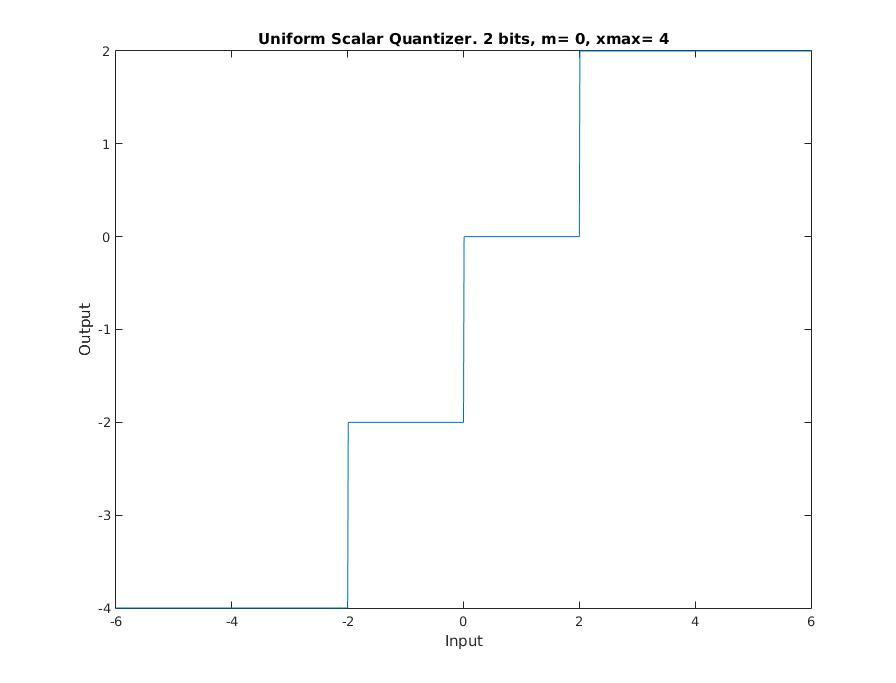
\includegraphics[scale=.3]{USQ_INOUT_m0} }
\subfloat[m = 1.5]{  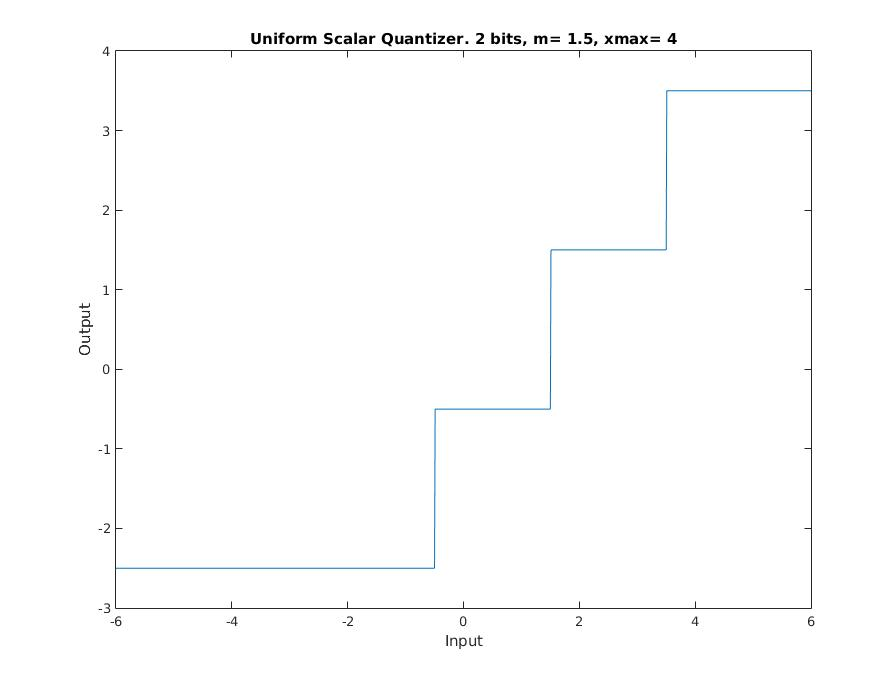
\includegraphics[scale=.3]{USQ_INOUT_m15} }

  \caption{Input vs Output}
  \label{USQ_INOUT}
\end{figure}
To compare the two settings, we need to plot the distorsion-rate curve and compare the performance. This is presented on figure \ref{USQ_RateDistCurve}.

\begin{figure}[!h]
  \centering
  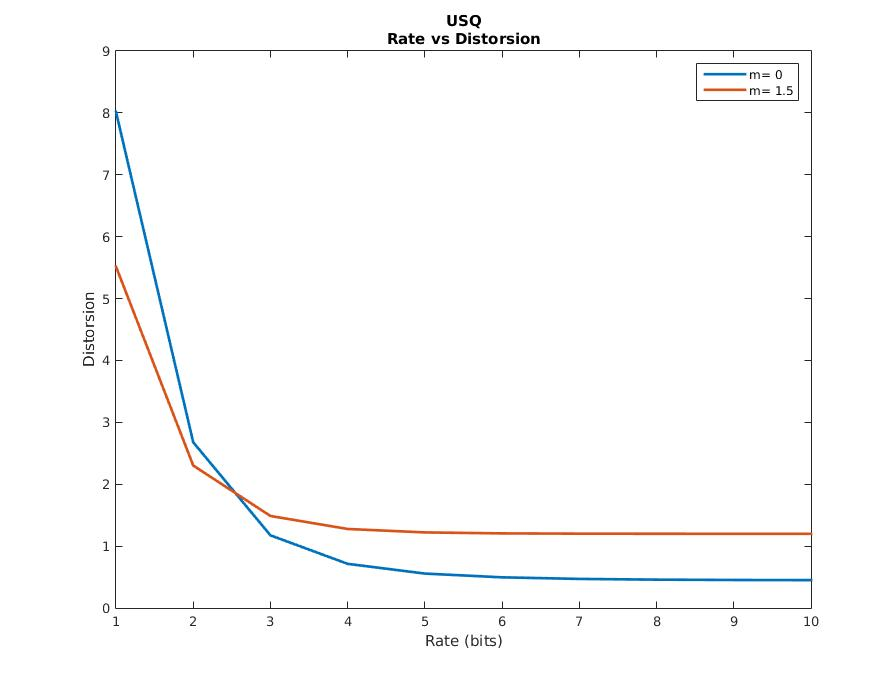
\includegraphics[scale=.35]{USQ_RateDistCurve}
  \caption{Rate-Distorsion curve for two values of m.}
  \label{USQ_RateDistCurve}
\end{figure}

%%% Local Variables:
%%% TeX-master: "master"
%%% End:
\pagebreak

\section{Parametric coding of speech}

In this part, we will experiment with parametric coding. We use the vocoder provided with the project for optimal performance.
With the analysis function we are able to get crucial parameters which describe the signal we want to transmit. This way we don't have to
transmit the whole signal which require a high number of bits. In order to use fewer bits, we will quantize the parameters before transmission.
The goal of this part is then to find a good ratio between quantization of the parameters and quality of the reconstructed received signal by
the synthesis function. The bitrate during transmission should be as low as possible while the quality of the signal on the reception side is
defined by the implementation (military, artistic, communication...).

In the following sections, we will analyse each parameter of the analysis function and try to find clever ways to quantize them.
We use the signal called \textit{male8}.

\subsection{Quantizing the Gain}

In this section, we work on the quantization of the gain.

\begin{figure}[h!]
\centering
\includegraphics[scale = .4]{histogram_gain}
\caption{Histogram of the gain with mean and boundaries}
\label{histgain}
\end{figure}

We apply a uniform quantizer on the gain with different bitrates then we synthesize the new signal. We cannot hear the distortion
above a 4 bits quantization. This means that we could use \textbf{4 bits window} to code the gain and the reconstructed signal would still have the same
quality as the original signal. 

We now compute and plot the histogram of the logarithm of the gain.

\begin{figure}[h!]
\centering
\includegraphics[scale = .4]{histogram_log_gain}
\caption{Histogram of the log of the gain with mean and boundaries}
\label{histloggain}
\end{figure}

We can see that the histogram here is more uniform. We can expect the quantization to better represent the variations of the log of the gain
compared to when used on the gain only. We apply the same test as before and find that we can go as far as quantizing the gain with 3 bits
and still not hear the distortion. We can observe the effect of these two methods of quantization by plotting the results along with the original
gain (Figure 5).

\begin{figure}[h!]
\centering
\includegraphics[scale = .4]{quantized_gain_3bits}
\caption{Comparison of original gain and quantized gains with 3 bits}
\label{histloggain}
\end{figure}

With \textbf{3 bits per window} we have 8 levels of quantization. We see that using a log quantization gives us logarithmically distributed levels of quantization,
therefore we are able to describe small variations in the lowest values. The direct quantization cannot do this.

In many ways, human speech and perception work logarithmically and not linearly. The pitch and the gain are examples of this. The quantization
in the log domain is better for those parameters.

\subsection{Quantizing the Pitch and Voiced/Unvoiced Decision}

\subsubsection*{Pitch}

As said previously, the pitch perception of human beings is logarithmic. Meaning that a logarithmic scale fits human pitch better than a linear one.
We will then quantize the pitch with the same method as the gain. With this method, we are able to achieve a quantization using \textbf{4 bits per window} with
little to no distortion.

\subsubsection*{Voiced/Unvoiced Decision}

The quantization of this parameter is very simple. Essentialy because this vector is binary by definition therefore does not need to be quantized more.
We can use only \textbf{1 bit per window} to code the values of this vector $\rightarrow$ bit set to 1 to indicate a voiced sample, bit set to 0 to indicate an unvoiced sample.

\subsection{Quantizing the LP parameters}

The quantization of the LP paramaters is inherently different than what has been done previously. We do not use a uniform scalar quantizer this time
but instead use a vector quantizer (VQ). We use an order of 10 to compute the LP parameters. This means that we have to transmit a vector of 10 scalars for each
window. Instead of coding the vector directly we will find within the VQ the closest vector (linked to a specific distance) and transmit its index. This means
that the coder and decoder both have to possess the VQ. We use 2 VQs: one that codes the coefficients directly, and one that codes the residual (the
error between the actual coefficients and the coefficients chosen by the coding function). This way we gain precision with only a small number of bits added.

The VQs store 1024 vectors of 10 coefficients. This means that any index within the list can be coded with 10 bits. We have to transmit 2 indexes for each window.
Therefore we need \textbf{20 bits per window} with this method.

We code 2 functions, \textit{encodefilter} and \textit{decodefilter} that both take the VQs as input. The first function finds, for each vector of coefficients, the
closest vector in the VQ1 using the euclidean distance. It computes the residual and codes it using VQ2 with the same distance. It outputs the 2 indexes for each window.
The second function finds, for each pair of indexes, the corresponding set of coefficients and adds them together to get a single vector. 

\subsection{Optimizing the Bit Allocation}

Now that we have quantized each parameter separately we can see the effect of quantizing all of them on the reconstructed signal. To sump up, here is a table
of the bitrate for each parameter.

\begin{figure}[h!]
\centering
\begin{tabular}{l*{4}{c}}
Number of bits			& bits/window	& bits/sample	& kbits/sec	\\
\hline
Gain (E)			& 3		& 0.0248	& 0.1987	\\
Voiced/Unvoiced (V)		& 1		& 0.0083	& 0.0662	\\
Pitch (P)			& 4		& 0.0331	& 0.2650	\\
LP Parameters (A)		& 20		& 0.1656	& 1.3248	\\
\hline \hline
Total				& 28		& 0.2318	& 1.8547	\\
\end{tabular}
\caption{Table of bitrates for \textit{male8} (length = 25242 samples = 3.15 sec)}
\end{figure}

We can see that the LP Parameters take indeed the largest portion of the bitrate.

We compute the SNR and get $SNR = 3.9 dB$. SNR is a great tool to describe the distortion that additive noise add to a signal or to describe
the distortion implied with quantization. However here we have to point out that we have quantized a set of parameters which served to synthesize
a new signal. Eventhough we want this signal to be as close as possible to the original signal, it might have some clear differences (delay, amplitudes,
periodicity...). Therefore the SNR here is not necessarily relevant to the quality of the signal.

%%% Local Variables:
%%% TeX-master: "master"
%%% End:


\pagebreak

\section{Speech Waveform Quantization}

%%% Local Variables:
%%% TeX-master: "master"
%%% End:
\pagebreak

\section{Adaptive Open-Loop DPCM}
In this section we have to implement an a Differential Pulse Code Modulator. The functional scheme is presented on figure \ref{dpmc}.
\begin{figure}[!ht]
\centering
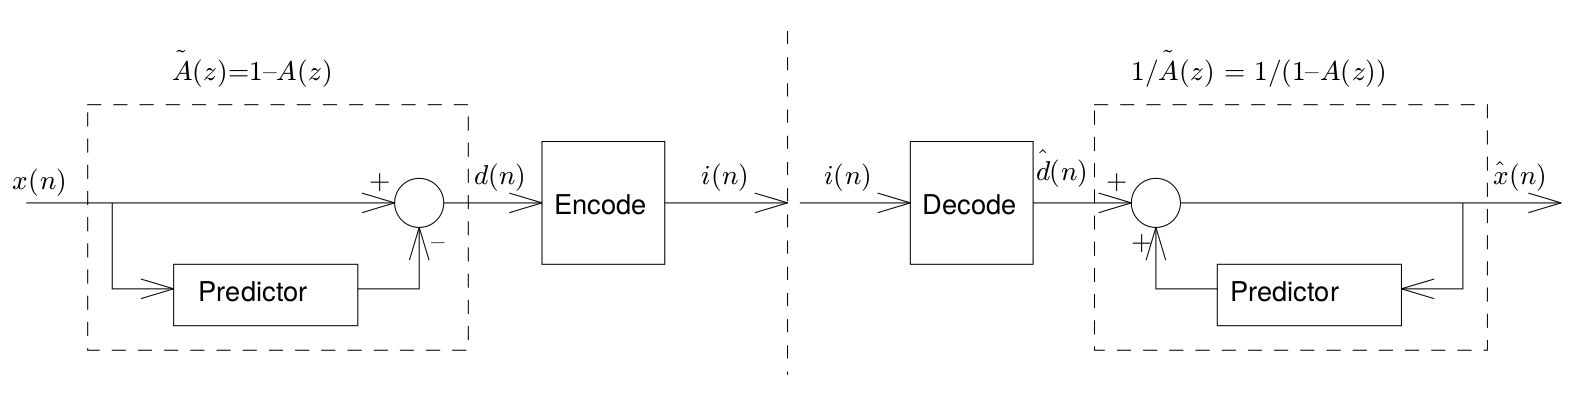
\includegraphics[scale=.3]{dpmc}
\caption{Functional scheme of a DPMC}
\label{dpmc}
\end{figure}

The idea here is to perform a linear prediction on an input signal, and to transmit the error signal with the prediction coefficient. It is not efficient to transmit a quantized input because the frames are strongly correlated between each other, as we can see on figure \ref{corr}.

\begin{figure}[!ht]
\centering
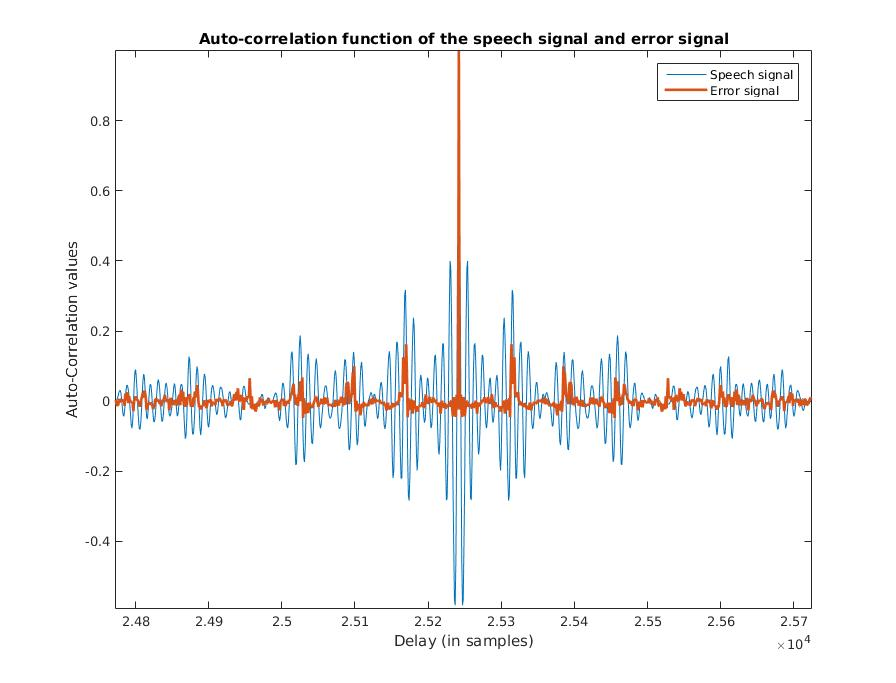
\includegraphics[scale=.4]{corr}
\caption{Correlation function of the input speech signal.}
\label{corr}
\end{figure}
%%% Local Variables:
%%% TeX-master: "master"
%%% End:


\pagebreak
\end{document}
